
%(BEGIN_QUESTION)
% Copyright 2013, Tony R. Kuphaldt, released under the Creative Commons Attribution License (v 1.0)
% This means you may do almost anything with this work of mine, so long as you give me proper credit

This diagram shows a sample system for a set of CEMS analyzers:

$$\includegraphics[width=15.5cm]{i03339x01.eps}$$

Identify and explain the consequence of a technician accidently leaving hand valve \#2 (V2) shut.  Assume everything else in this analyzer system is operating as it should.

\vskip 50pt

Identify and explain the consequence of the backpressure regulator R6 failing wide open (venting fully all the time).  Assume everything else in this analyzer system is operating as it should.  

\vskip 50pt

\underbar{file i03339}
%(END_QUESTION)





%(BEGIN_ANSWER)

Identify and explain the consequence of a technician accidently leaving hand valve \#2 (V2) shut.  Assume everything else in this analyzer system is operating as it should.  {\bf The CO analyzer will not be able to get its span gas properly to auto-calibrate.  Thus, its calibration will likely drift off of spec over time.}

\vskip 10pt

Identify and explain the consequence of the backpressure regulator R6 failing wide open (venting fully all the time).  Assume everything else in this analyzer system is operating as it should.  {\bf None of the analyzers will receive enough sample gas pressure to properly operate.  The gas samples inside of them will be stagnant with the last calibration gas sample sent to each analyzer (could be zero, could be span).}

\vskip 10pt

I recommend granting half-credit for each correct explanation (5 points each).

%(END_ANSWER)





%(BEGIN_NOTES)

{\bf This question is intended for exams only and not worksheets!}.

%(END_NOTES)

